\documentclass[10pt]{beamer}
    
    \usetheme{glasgow}
    
    \usepackage{booktabs}
    \usepackage[scale=2]{ccicons}
    \usepackage{minted}
    \usepackage{bookmark}
    \usepackage[style=verbose]{biblatex}
    % \usepackage{filecontents}% to embed the file `myreferences.bib` in your `.tex` file
    % \begin{filecontents*}{refs.bib}
    %     @misc{schneider_understanding_nodate,
    %     title = {Understanding the {FDTD} {Method}},
    %     url = {https://eecs.wsu.edu/~schneidj/ufdtd/},
    %     author = {Schneider, John}
    % }
    % \end{filecontents*}

    \addbibresource{refs.bib}

    % \usepackage[noadjust]{cite}
    \usepgfplotslibrary{dateplot}
    
    \usemintedstyle{trac}
    
    % ($ (A)!r!(B) $) the location of images to be used
    \graphicspath{{src/}}
    
    %% Customisation
    % \newcommand{\V}[1]{\v} % vectors \v{c}
    % \renewcommand{\v}[1]{\mathbf{#1}} % vectors
    \newcommand{\ti}[1]{\tilde{#1}} % spectral representation
    \newcommand{\tnsr}[1]{\underline{\underline{#1}}}
    
    % Symbols
    \renewcommand{\O}{\omega}  % omega
    \newcommand{\E}{\varepsilon}  % epsilon
    \renewcommand{\u}{\mu}  % mu
    \newcommand{\p}{\rho}  % rho
    \newcommand{\x}{\times}  % times
    \renewcommand{\inf}{\infty}  % infinity
    \newcommand{\infint}{\int\limits_{-\inf}^\inf} % integral by R
    \newcommand{\e}{\mathrm{e}} % Straight-up exponential
    \renewcommand{\j}{{j}\mkern1mu} % Straight-up exponential
    \newcommand{\iu}{\mathrm{i}\mkern1mu}
    
    \newcommand\ddfrac[2]{\frac{\displaystyle #1}{\displaystyle #2}}
    
    \usepackage{animate}



%     % Define a the counter cnt. Used to identify files generated for use
% % with Gnuplot.
% \newcounter{cnt}
% \setcounter{cnt}{0}

% % Macro for drawing one frame of the F-distribution animation.
% \newcommand{\fdst}[4]{%
%     % shade the critical region tail
%     \draw[fill,orange]  (#1,0) -- plot[id=5\thecnt,domain=#1:5.5,samples=50]
%         function {#4*(x**(0.5*#2-1))*((1+#2*x/#3)**(-0.5*#2-0.5*#3))}
%             -- (5.5,0) -- cycle;

%     % draw the F distribution curve
%     \draw[color=blue!50!black,thick]
%         plot[id=f4\thecnt,smooth,domain=0:5.5,samples=100]
%         function {#4*(x**(0.5*#2-1))*((1+#2*x/#3)**(-0.5*#2-0.5*#3))};

%     % draw the F axis
%     \draw[->] (0,0) -- (6,0) node[right] {$F$};
%     % label the critical region boundary
%     \draw (#1,0) -- (#1,-0.02) node[below] {$#1$};
%     % label 0
%     \draw (0,0) -- (0,-0.02) node[below] {$0$};

%     % add some lables for degrees of freedom and alpha level
%     \draw (2,0.5) node[right] {$df_1 = #2$};
%     \draw (2,0.4) node[right] {$df_2 = #3$};
%     \draw (2,0.3) node[right] {$\alpha = 0.10$};

%     % draw the y axis
%     \draw[very thin,->] (0,0) -- (0,0.8);
% }


    \title{High Frequency Communication Systems}
    \subtitle{Lecture 7}
    \date{Spring 2021}
    \author{Hasan T Abbas \& Qammer H Abbasi}
    % \institute{}
    




\begin{document}

\maketitle

%%%%%%%%%%%%%%%%%%%%%%%%%%%%%%%%%%%%%%%%%%
%%%%%%%%%%%%%%%%%%%%%%%%%%%%%%%%%%%%%%%%%%
%%%%%%%%%%%%%%%%%%%%%%%%%%%%%%%%%%%%%%%%%%
\begin{frame}[fragile]
    \frametitle{Lecture Outline}
    \begin{outline}[itemize]
        \1 Antenna Arrays
        \1 Array Analysis
        \1 Mutual Coupling between Array elements
    \end{outline}
\end{frame}
%%%%%%%%%%%%%%%%%%%%%%%%%%%%%%%%%%%%%%%%%%
%%%%%%%%%%%%%%%%%%%%%%%%%%%%%%%%%%%%%%%%%%
%%%%%%%%%%%%%%%%%%%%%%%%%%%%%%%%%%%%%%%%%%

\section{Antenna Arrays}




\begin{frame}
    \frametitle{Antenna Array Motivation}

    \begin{columns}[T]
        \begin{column}{.4\textwidth}
            \begin{outline}
                \1 In individual antenna elements, we can't control the radiation patterns
                \1 If we \textit{combine} two antenna elements, it is possible to change the pattern significantly
                \2 We call the new combined structure as an \textcolor{red}{antenna array}.
                \1 We achieve higher directivity using antenna arrays
            \end{outline}
        \end{column}
        \begin{column}{.6\textwidth}
            \begin{figure}[h!]
                \centering
                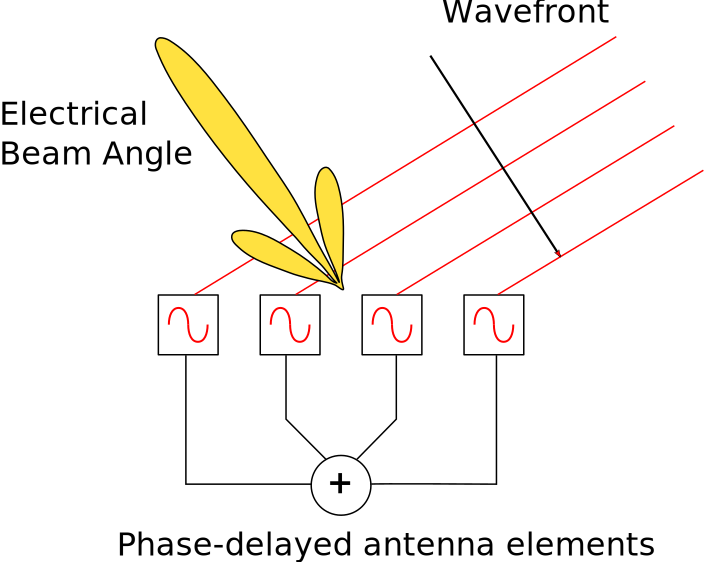
\includegraphics[width=0.95\textwidth]{antenna_array.pdf}
                \caption{Typical antenna array with phased elements.}
            \end{figure}
        \end{column}
    \end{columns}
        
\end{frame}



\begin{frame}
        \frametitle{Antenna Array Applications}
        \begin{columns}[T]
            \begin{column}{.4\textwidth}
                \begin{outline}
                    \1 Communications Applications
                    \2 The goal is to focus EM energy towards the target population (cars, people, cities etc.)
                    \3 Modern wireless communications using beamforming
                    \1 Radar - multiple target tracking
                    \2 We would like to focus the energy on the targets as they move
                \end{outline}
            \end{column}
            \begin{column}{.6\textwidth}
                \begin{figure}[h!]
                    \centering
                    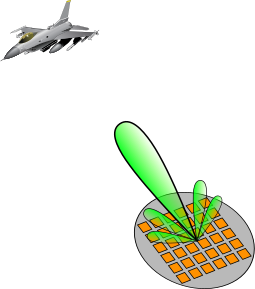
\includegraphics[width=0.65\textwidth]{arrays_motivation.pdf}
                    \caption{A Phased array antenna in RADAR based target tracking.}
                \end{figure}
            \end{column}
        \end{columns}

\end{frame}

\begin{frame}
    \frametitle{The Array element - point dipole}
    \begin{columns}[T] % align columns
        \begin{column}{.4\textwidth}
            \begin{outline}
                \1 Recall from the antenna introduction lecture, the field pattern of an infinitesimal dipole:
            \end{outline}
            \begin{align*}
                \va{E} {}=& \vu*{\gamma} \j k \eta I_0 l \frac{\exp(-\j k r)}{4 \pi r} \sin \gamma \nonumber \\
                &= \j k \eta \va{h} G(r)
            \end{align*}
            where $\va{h} = \vu*{\gamma} I_0 l \sin \gamma$ and $G(r)$ is the free-space Green function for a point source, $\exp(\j k r)/(4 \pi r)$
            \begin{outline}
                \1 We will use this as the antenna element
            \end{outline}
        \end{column}
        \begin{column}{.4\textwidth}
            \begin{figure}[B!]
                \centering
                \includegraphics[width=.75\textwidth]{line_source.pdf}
            \end{figure}
            \begin{figure}[h!]
                \centering
                \includegraphics[width=.9\textwidth]{3d_pattern.pdf}
            \end{figure}
        \end{column}%
    \end{columns}
\end{frame}

\begin{frame}
    \frametitle{Obtaining a desired pattern}

    \begin{outline}
        \1 There are some factors that determine the desired radiation pattern
        \2 Array Geometry
        \2 Element Spacing
        \2 Element Excitation Amplitude
        \2 Pattern of individual element
    \end{outline}
The total field is given by:
\begin{align*}
    E_{total} {}=& \mathrm{Element \, \, Factor}  \times \mathrm{Array \, \, Factor}
\end{align*}
\end{frame}

\begin{frame}
    \frametitle{Two Element Array}
    \begin{columns}[T] % align columns
        \begin{column}{.6\textwidth}
            \begin{outline}
                \1 The simplest antenna array contains two elements
                \1 Two analyse an array, we start by using point sources as individual elements
                \2 The final pattern is obtained by multiplication
                \1 First, we will ignore the mutual coupling between elements.
                \1 Consider an array of two point sources separated by a distance $d$ on the $y$-axis.
            \end{outline}
            \begin{outline}
                \1 Assuming that both the antenna elements are excited by the current $I_1 = I_0 \exp (\j \alpha/2)$ and $I_2 = I_0 \exp (-\j \alpha/2)$ where $0 \le \alpha \le 2 \pi$.
            \end{outline}   
        \end{column}
        \begin{column}{.4\textwidth}
            \begin{figure}[T!]
                \centering
                \includegraphics[width=.8\textwidth]{two_elements.pdf}
                \caption{Two point sources forming a basic antenna array.}
            \end{figure}

        \end{column}%
    \end{columns}
\end{frame}


\begin{frame}
    \frametitle{Two element array - Total Fields}
Neglecting any mutual coupling, we obtain the total fields by simple vector summation:
\begin{align*}
    \va{E_t} {}=& \va{E_1} + \va{E_2} \\
    &= \vu*{\gamma} \j \beta \eta \frac{I_{0} \ell}{4 \pi}\left\{\frac{\e^{-\j \beta R_{1}}}{R_{1}} \e^{+\j \alpha / 2} \sin \gamma_{1}+\frac{\e^{-\j \beta R_{2}}}{R_{2}} \e^{-\j \alpha / 2} \sin \gamma_{2}\right\}
 \end{align*}
    We use the \textit{far-field} approximation:
    \begin{align*}
        \Gamma_1 \approx \Gamma_2 \approx \Gamma \\
        R_1 \approx r - \frac{d}{2} \cos \theta \\
        R_2 \approx r + \frac{d}{2} \cos \theta \\
       R_1 \approx R_2 \approx r (\mathrm{amplitude \, term})
    \end{align*}
\end{frame}

\begin{frame}
    \frametitle{Two element array - Total Fields}

    The total \textit{far-field} thus becomes:
    \begin{align*}
        \va{E_t} {}=& \vu*{\gamma} \j \beta \eta \frac{I_{0} \ell}{4 \pi r} \sin \gamma \left\{\e^{-\j \beta \frac{d}{2}\cos \theta } \e^{- \j \alpha / 2} + \e^{-\j \beta \frac{d}{2}\cos \theta } \e^{+\j \alpha / 2}\right\} \\
        &= \j \beta \eta \va{h} G(r) \left\{ \e^{\frac{\beta d cos \theta + \alpha}{2}} + \e^{-\frac{\beta d cos \theta + \alpha}{2}}\right\} \\
        &= \underbrace{\j \beta \eta \va{h} G(r)}_{Element \, Factor} \underbrace{2 \cos \left[\frac{1}{2}\left(\beta d \cos \theta + \alpha\right)\right]}_{Array \, Factor}
    \end{align*}
We can control and change the pattern by varying $d$ and $\alpha$, that are the spacing and phase shifts
\end{frame}




% \begin{frame}[fragile]
%     \frametitle{Final Expressions}
%     \begin{figure}[h!]
%         \centering
%         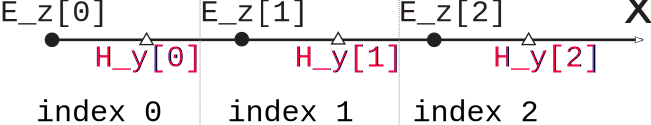
\includegraphics[width=.7\textwidth]{code_fdtd_1d.pdf}
%         \caption{Array variable definition for 1D FDTD.}
%     \end{figure}
%     The update equations for a computer program therefore are:
%     \begin{minted}{python}
%     hy[i] = hy[i] + (ez[i + 1] - ez[i]) / imp0

%     ez[i] = ez[i] + (hy[i] - hy[i - 1]) * imp0
% \end{minted}
%     Here \texttt{imp0} is the characteristic impedance, and $S_c = 1$ is assumed 1. Note the magnetic field is calculated first and then the electric field. We place the expressions above in a loop.
% \end{frame}



% %% example of an ANIMATED FRAME
% % \begin{frame}

% %         \begin{animateinline}[autoplay]{20}
% %             \multiframe{21}{rXmax=0+0.1}{
% %               \begin{tikzpicture}
% %               \begin{axis}[
% %                 axis lines=center,
% %                 domain=0.001:\rXmax,
% %                 xtick={0,1,...,8},
% %                 xmax=8.4,
% %                 ymax=1.6,
% %                 samples=51
% %               ]
% %               \addplot [gray, dashed] {1};

% %               \addplot [color=red] {1-exp(-x)*cos(3*deg(x))};

% %               \end{axis}
% %               \end{tikzpicture}
% %             }
% %             \end{animateinline}

% %   \end{frame}


\end{document}
